\refstepcounter{sdel}
\section{Scientific Deliverable \thesdel\ -- What is a Microservice?}
{\color{gray}
For each scientific deliverable targeted in section~\ref{sec-deliverables} provide a full section with all the subsections described below.
\label{sec-production}
}

\subsection{Requirements (± 15\% of section's words)}
% {\color{gray}
% Describe here all the properties that characterize the deliverables you produced. It should describe, for each main deliverable, what are the expected functional and non functional properties of the deliverables, who are the actors exploiting the deliverables. It is expected that you have at least one scientific deliverable (e.g. ``Scientific presentation of the Python programming language'', ``State of the art on quality models for human computer interaction'', \ldots.) and one technical deliverable (e.g. ``BSProSoft - A python/django web-site for IT job offers retrieval and analysis'', \ldots). 
% }

Since \glspl{ms} were a previously unknown concept to me, this
scientific deliverable targets the familiarisation of this
architectural style. In the design section we are going to elaborate
on motivations behind the architecture.  In the production we will
explore what constitutes a \gls{ms} and the assessment will highlight
a few drawbacks of the \gls{ms} architecture.

\subsection{Design (± 30\% of section's words)}
% {\color{gray}
% Provide the necessary and most useful explanations on how those deliverables have been produced.
% }

To understand the benefits and motivations behind using \gls{ms} over
the monolithic style, we will first look at the latter.
\cite{ms-definition}

Monolithic architectures build applications using a single unit. This
basically means that all of an application's functionality, logic,
classes, function and name spaces are in the end located within a
single executable and thus run within a single process. This model is
very much usable in fact and allows us to create functioning
systems---as has demonstrated the time of software development before
\glspl{ms} were introduced. However, this architectural style raises
some issues nonetheless. For instance, even the smallest of changes in
an application require the whole product to be rebuilt and redeployed
or redistributed which is not necessarily an ideal scenario.

As the application's life cycles goes on, it is unavoidable to modify
it over time. In a monolithic system however, it becomes increasingly
difficult to maintain a modular structure---if one was present to
begin with---which in turn also leads to modifications becoming more
expensive. The expensive modifications are explained by the fact that
if a modular structure cannot be guaranteed, it possibly entails that
changes to one component may impact other components which were not
supposed to be affected. This may result in many adjacent changes and
unexpected issues to be performed and treated respectively.

Lastly, if we want to scale an application we actually need to scale
the application as a whole rather than the individual components that
need to be scaled.

\begin{figure*}
	\centering
	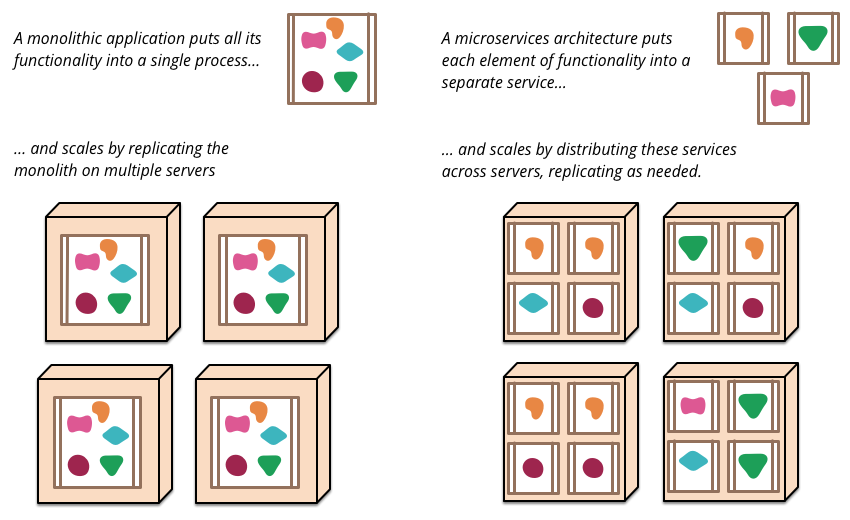
\includegraphics[width=0.75\linewidth]{images/sketch.png}
	\caption{Monoliths and Microservices}
	\label{fig:monoliths-ms}
\end{figure*}

Figure \vref{fig:monoliths-ms} nicely demonstrates some of the
mentioned issues and how the \gls{ms} architecture tries to tackle
them.

Since the application is now split into separate services, making
modifications will not require us to build and deploy the whole
application anew. It will be enough to only update the services in
question.

Further, the fact that the application is built in a modular fashion
from the ground up and divided into smaller chunks and services, makes
it easier to maintain a modular structure within the application as a
whole. As a result, making changes to one such service will guarantee
that none of the other services will be affected and thus keep
undesired or unforeseen side effects to a minimum.

We can also see that scaling an application becomes much less of a
burden. No longer do we need to scale the whole application, but we
can simply introduce new services where needed.

\subsection{Production (± 40\% of section's words)}
% {\color{gray}
% Provide descriptions of the deliverables concrete production. It must present part of the deliverable (e.g. source code extracts, scientific work extracts, \ldots) to illustrate and explain its actual production.
% }

A first simple definition can be found in the MSs article
\cite{ms-definition} that lays out some aspects which characterize a
MS architecture.

\begin{quote}
	In short, the microservice architectural style is an approach to
	developing a single application as a suite of small services,
	each running in its own process and communicating with
	lightweight mechanisms [\ldots]. These services
	are built around business capabilities and independently
	deployable by fully automated deployment machinery. There is a
	bare minimum of centralized management of these services, which
	may be written in different programming languages and use different
	data storage technologies. 
\end{quote}

However, as stated multiple times in the article \cite{ms-definition},
there is no formal definition for MS. As such, we shall inspect
characteristics that such architectures tend to have in common.

Before we move on, an interesting point to note here is the decreased
need for \textit{centralized management}. To give an example
\cite{central-decentral}, centralized management is a structure where
only a few individuals make most of the decisions in a company. We can
find hierarchies within such a structure, each having to respond to
the superior's communicate. 

Decentralized management on the other hand would for example allow a
manager at a call center or retail store to make instant decisions
that impact their work environment. Thus, the decisions are not taken
solely by the higher ups but responsibilities are spread across
sectors—which could further spread responsibilities. This is an
interesting analogy to keep in mind for the following.

\subsubsection{Componentization via Services}

The article \cite{ms-definition} distinguishes between two types of
components---where \textit{component} refers to a unit of software
that is independently replaceable and upgradeable:

\begin{description}
	\item[libraries] which are being linked into a program and are
		called using in-memory function calls; and
	\item[services] which are external components where communications
		happen with mechanisms such as web service requests or remote
		procedure calls.
\end{description}

The advantage of \textit{services} is that such components can be
deployed independently---which is not the case with \textit{libraries}
because then a component is essentially directly integrated into
another component. It should be noted that some service component
modifications may affect its interface, which in turn will require
other service components to be adjusted accordingly. The aim however
is to minimize these through cohesive service boundaries and evolution
mechanisms in the service contracts.

Another advantage of services is a more explicit component interface.
Often it's only documentation and discipline that prevents clients
from breaking a component's encapsulation, thus leading to
overly-tight coupling between components. Services make it easier to
avoid this by using explicit remote call mechanisms.

\subsubsection{Organized around Business Capabilities}

Traditionally, splitting a large application into parts is done by
assigning a specialized team to each layer of the application, as
illustrated in figure \ref{fig:conway}. This distribution of work force
eventually leads to each team worrying only about their specific task
instead of the application as a whole, which is an example of
\textit{Conway's Law}:  

\begin{quote}
	Any organization that designs a system (defined broadly) will
	produce a design whose structure is a copy of the organization's
	communication structure.  
\end{quote}

\begin{figure}
	\centering
	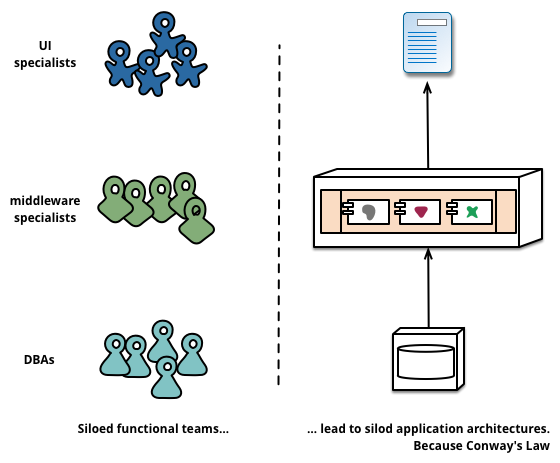
\includegraphics[width=\linewidth]{images/conways-law.png}
	\caption{Conway's Law in action}
	\label{fig:conway}
\end{figure}

In regards to MS, we divide the work force according to
\textit{business capabilities} rather than application layers. This
implies that our resulting team will be
cross-functional\footnote{meaning that our team is comprised of people
with different expertises, all working closely together for a common
goal}, combining the full range of skills required to develop the
service in question. This division leads us to figure
\vref{fig:team-boundaries}.

\begin{figure}
	\centering
	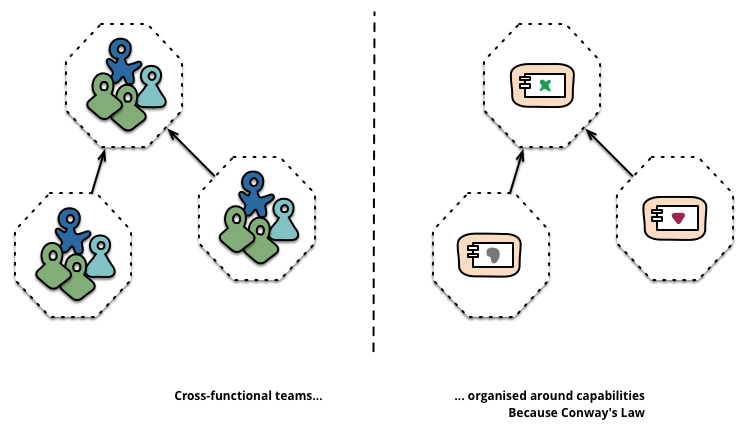
\includegraphics[width=\linewidth]{images/PreferFunctionalStaffOrganization.png}
	\caption{Service boundaries reinforced by team boundaries}
	\label{fig:team-boundaries}
\end{figure}

\subsubsection{Products not Projects}

Most of the application development focuses on delivering a piece of
software which is then considered completed. It is then handed over to
a separate maintenance team and the original team that built it will
then completely abandon the project.

The \gls{ms} philosophy tries to avoid this approach and instead
considers that a team should be responsible for its own product over
the full lifetime. Here is also a link to \textit{business
capabilities} in that software is no longer considered as a set of
functionalities that need to be completed. Rather it is seen as an
on-going relationship where one strives to enhance the business
capabilities by having the software assist its users.

\subsubsection{Smart endpoints and dumb pipes}

Often times when it comes to process communication, great importance
is put on the communication mechanism itself. With regards to
microservices however, we place greater importance on the endpoints
rather than the pipes.

Thus one should strive to decouple the \glspl{ms} and keep them as
cohesive as possible. One could almost say that they follow the Unix
philosophy in that they receive a request, treat it appropriately, and
then return a response. \gls{ms} can achieve this by using simple
REST-like protocols.

This further highlights that services in a microservice architecture
are to be isolated components. When they communicate, the
magic happens on the services' endpoints and not in the message
bus---in fact we need nothing more for messages than simply being
transferred from one endpoint to the other.

\subsubsection{Decentralized Governance}

Centralized governance that often comes along with monolithic
architectures have the tendency to standardize on single technology
platforms, which can be restricting. Rarely can a single language's
full potential be leveraged for the entirety of an application.

Splitting our application into services however, we do have the
ability and choice of building each service with whatever tool is best
for the job.

This approach also brings a different mindset into development.
Instead of focusing solely on defined standards for a product,
developers prefer the idea of creating useful tools that can
potentially also be used by other developers to solve similar
problems.

\subsubsection{Decentralized Data Management} 

Monolithic applications usually prefer to have a single logical
database for persistent data, which in turn are then often used across
a range of applications. Microservices on the other hand let each
service manage its own database. Both situations are illustrated in 
figure \vref{fig:databases}.

The issue that arises with decentralizing the data, however, is
consistency.  Managing this is in fact not an easy task and usually
comes at the cost of increased computing times, leading to
\textit{eventual consistency} and \textit{compensation operations}
being the preferred method.  In fact, businesses are often capable of
handling a degree of inconsistency in favor of quick responses to
demands.

\begin{figure}
	\centering
	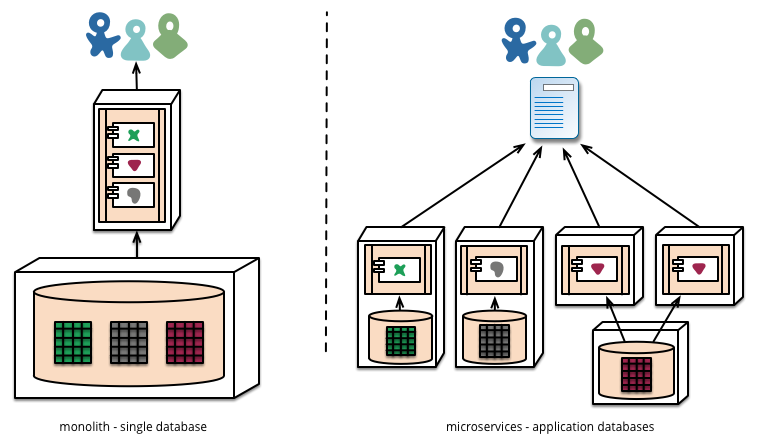
\includegraphics[width=\linewidth]{images/decentralised-data.png}
	\caption{Monolith and Microservice Databases}
	\label{fig:databases}
\end{figure}

\subsubsection{Infrastructure Automation}

Many products following the \gls{ms} architecture make heavy use of
\gls{cicd} and infrastructure automation tools. This becomes
especially relevant in production when you have to manage a lot of
different \glspl{ms} at once, which simply becomes infeasible without
the automation.

\subsubsection{Design for failure}

One needs to take into consideration that a service may fail at any
point in time for whatever reason, and the client should respond to
this as gracefully as possible. Due to the decoupled nature of
\glspl{ms}, we have an additional complexity to take into account
which constantly requires us to reflect on how service failure can
affect the user experience.

It is therefore of utmost importance to detect failures quickly and
restore the service. To achieve this, a lot of sophisticated
monitoring and logging on various parts of a service are performed.


\subsection{Assessment (± 15\% of section's words)}
% {\color{gray}
% Provide any objective elements to assess that your deliverables do or do not satisfy the requirements described above. 
% }

\KB{Talk about drawbacks}

\KB{Highlight elements pointing to TD}
